% !TeX program = xelatex
\documentclass{zjureport}
\special{dvipdfmx:config z 0} % 取消PDF压缩,加快速度,最终版本生成的时候最好把这句话注释掉

% =============================================
% Part 0 Edit the info
% =============================================

\major{电子科学与技术}
\name{韩寒、谌梓轩}
\partner{}
\title{本科实验报告}
\stuid{Group 6}
\college{信息与电子工程学院}
\date{\today}
\lab{东四221}
\course{电子电路设计实验2}
\instructor{王子立}
\grades{}
\expname{电设2课程设计报告}
\exptype{}


\begin{document}
	% =============================================
	% Part 1 Header
	% =============================================
	\makecover
	
	\makecontent
	
	%\makeheader
	% =============================================
	% Part 2 Main document
	% =============================================
	
	
	\section{ECG信号检测调理电路}
	
	\subsection{电路装配调试步骤}
	
	<1>前期PCB版图设计。在实际进行ECG心电信号测试之前,我们先对心电信号处理电路进行原理图设计,并生成PCB图,在仿真过程中,保证其能够正常工作并达到预期效果。
	
	<2>demo板焊接。根据元件装配表,依次进行元件的焊接,并在最后插上运算放大器和芯片。
	
	<3>进行低通滤波部分的测试。将示波器的传输线勾在TP2的针脚和GND上,设置波形发生器从20Hz到140Hz每隔20Hz依次增大,观察示波器上的波形变化,并记录峰峰值。
	
	<4>进行高通滤波部分的测试。将示波器的传输线勾在TP4的针脚和GND上,设置波形发生器从20mHz到80mHz每隔20mHz依次增大,观察示波器上的波形变化,并记录峰峰值。
	
	<5>进行陷波部分的测试。将示波器的传输线勾在TP9和GND上,设置波形发生器从20Hz到140Hz每隔20Hz依次增大,观察示波器波形,记录峰峰值。
	
	<6>进行总体放大性能的测试。将示波器的传输线勾在TP11和GND上,设置波形发生器从20Hz到140Hz每隔10Hz依次增大,观察示波器波形,记录峰峰值。
	
	\subsection{电路测试数据分析}
	
	\subsubsection{低通滤波部分}
	
	在测试低通滤波部分的效果时,我们主要测试20Hz到140Hz部分,部分测试图如图\ref{低通滤波20Hz}、\ref{低通滤波60Hz}、\ref{低通滤波100Hz}、\ref{低通滤波140Hz}所示,测量结果如表\ref{低通滤波20Hz到140Hz测量结果}所示。
	
	\begin{figure}[h]
		\centering
		\begin{minipage}[t]{0.49\linewidth}%%%%%%%%%note2
			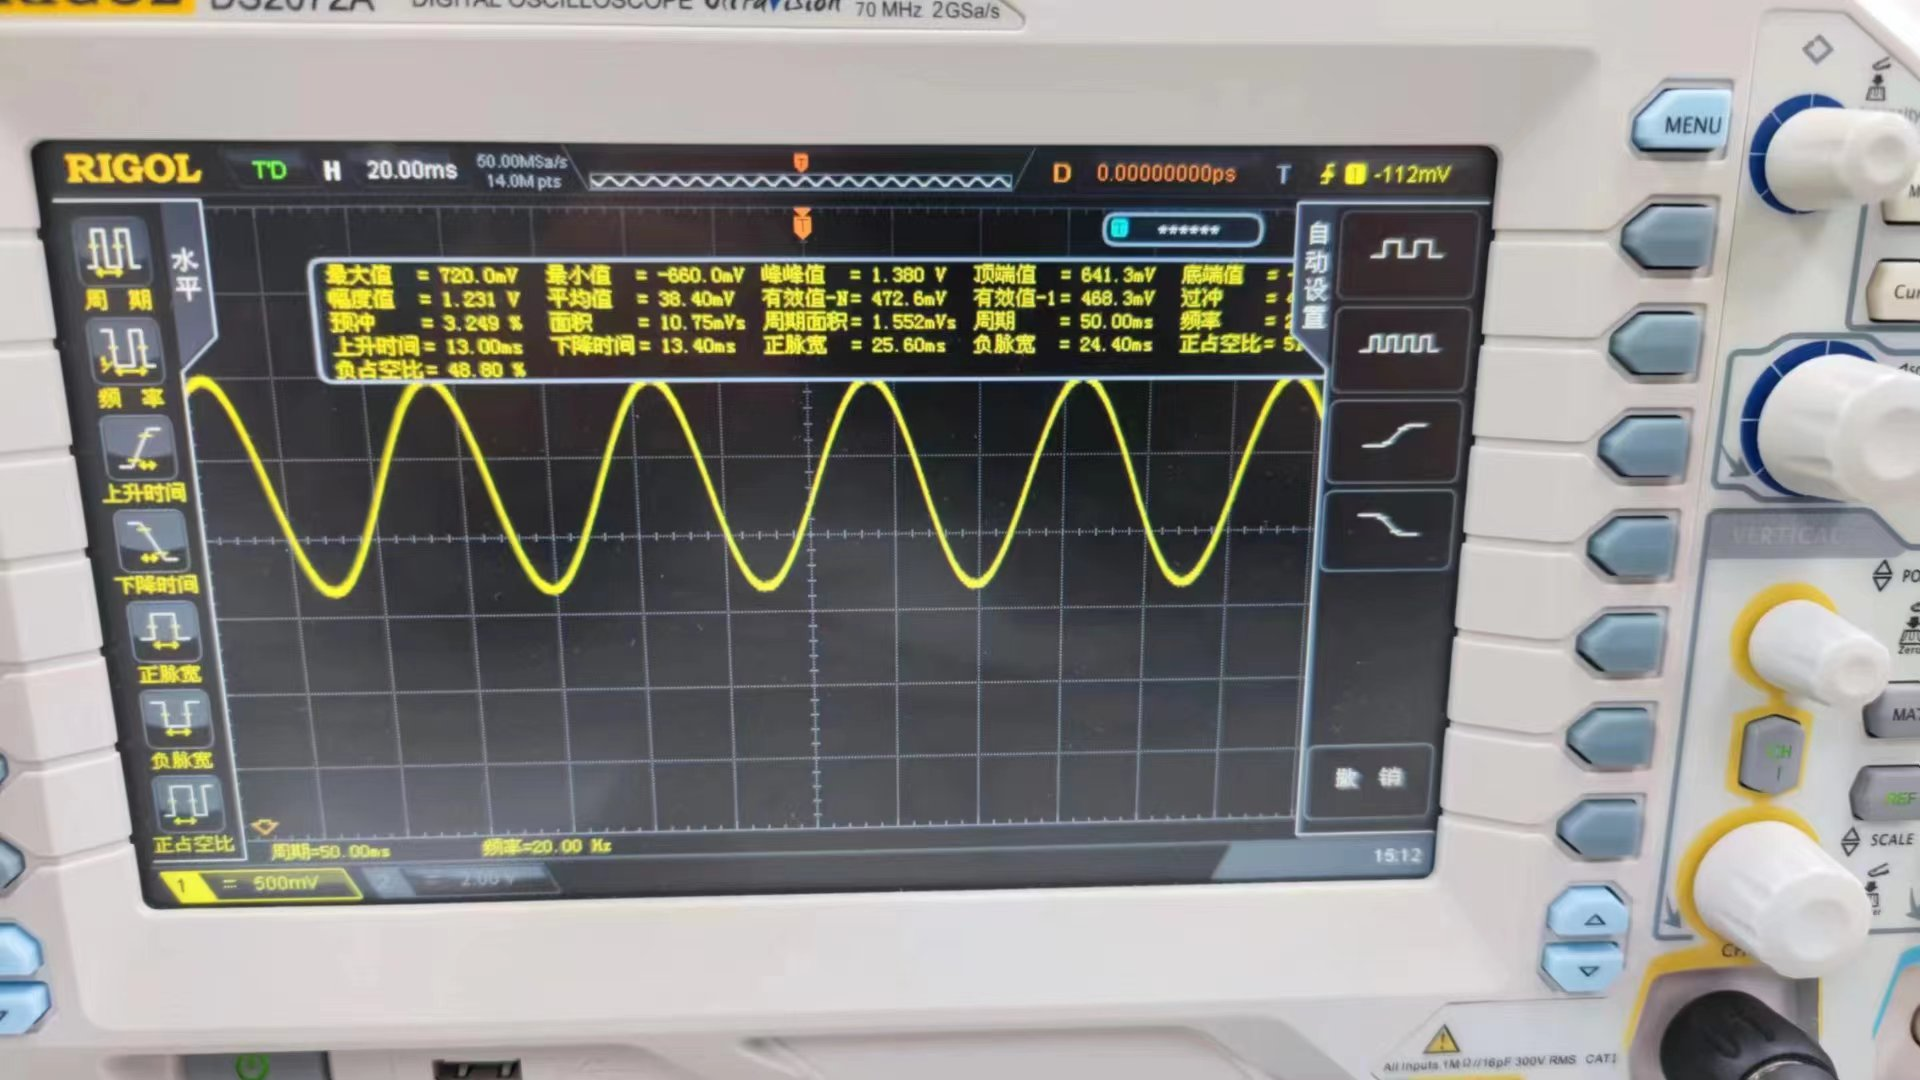
\includegraphics[width=0.9\linewidth]{低通滤波20Hz}%%%%%%%%%note3
			\caption{低通滤波20Hz}
			\label{低通滤波20Hz}
		\end{minipage}%
		\begin{minipage}[t]{0.49\linewidth}
			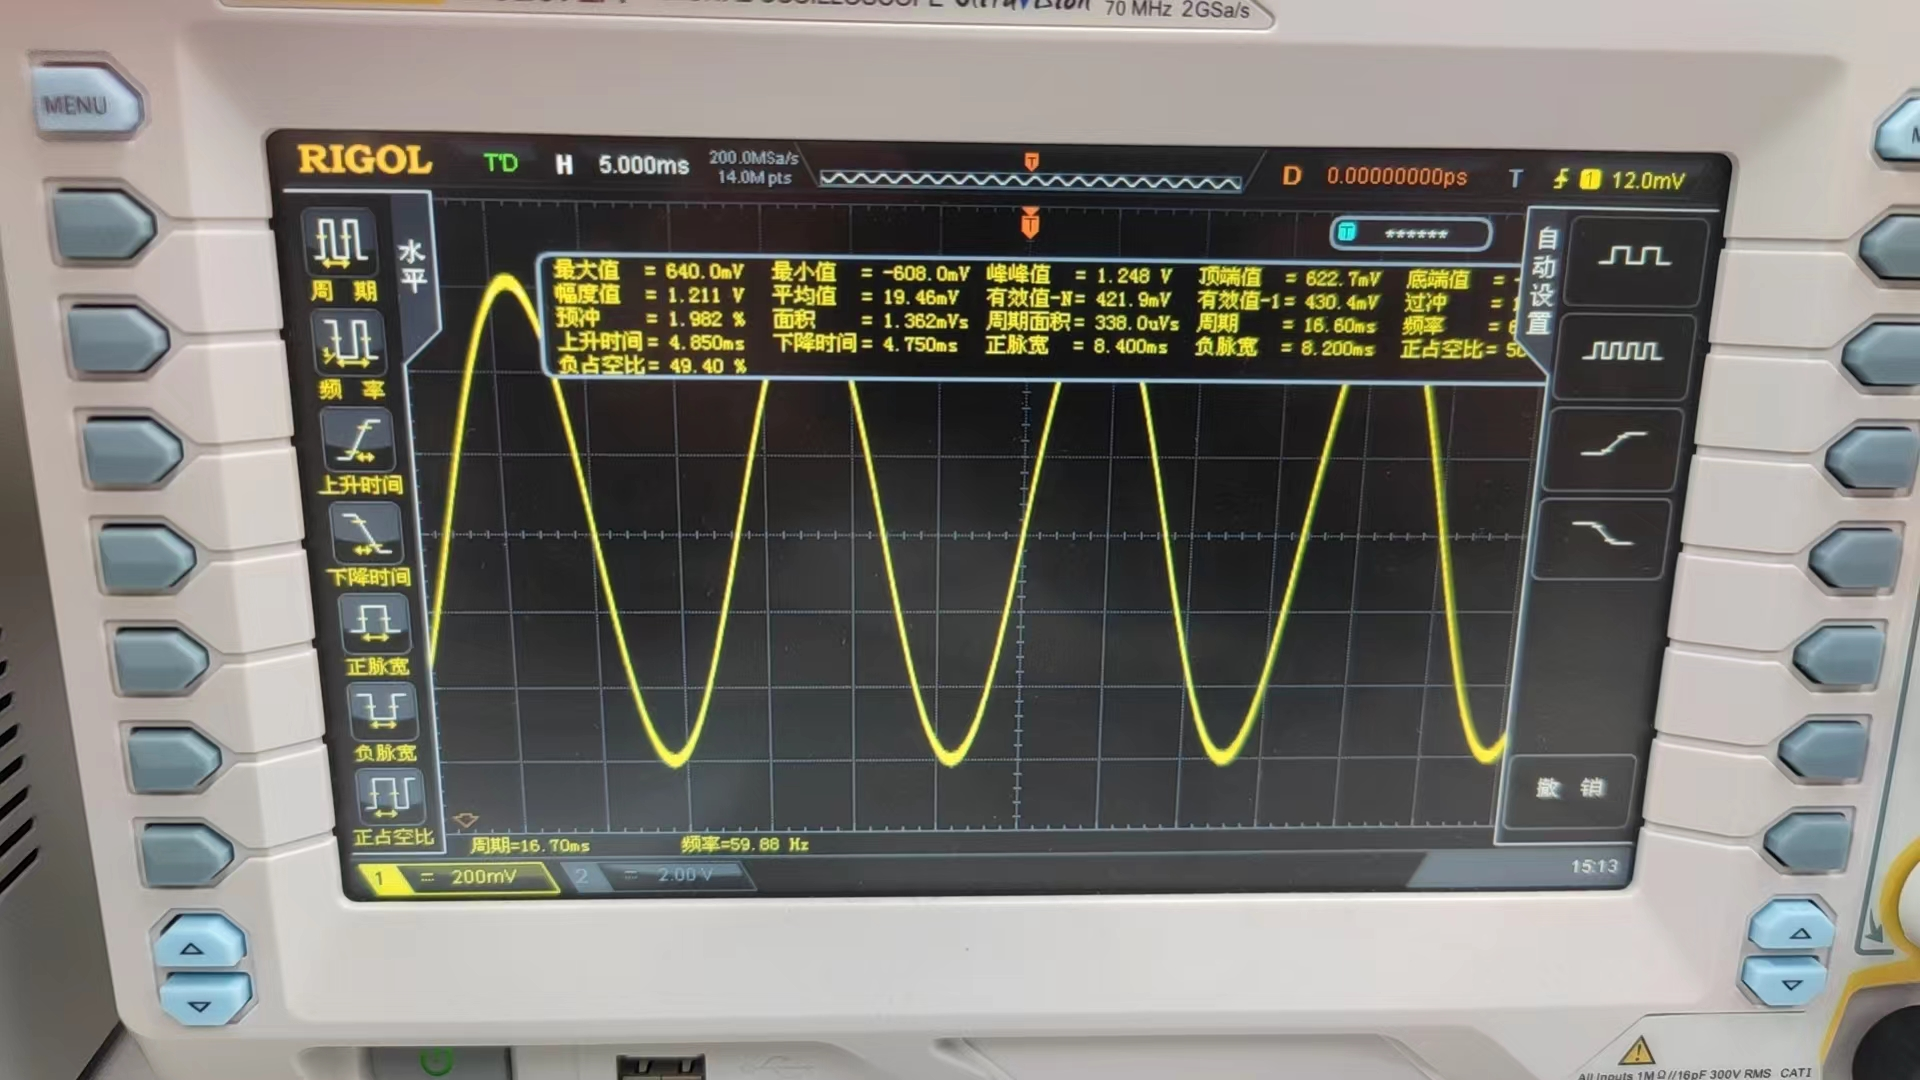
\includegraphics[width=0.9\linewidth]{低通滤波60Hz}
			\caption{低通滤波60Hz}
			\label{低通滤波60Hz}
		\end{minipage}
	
		\begin{minipage}[t]{0.49\linewidth}%%%%%%%%%note2
			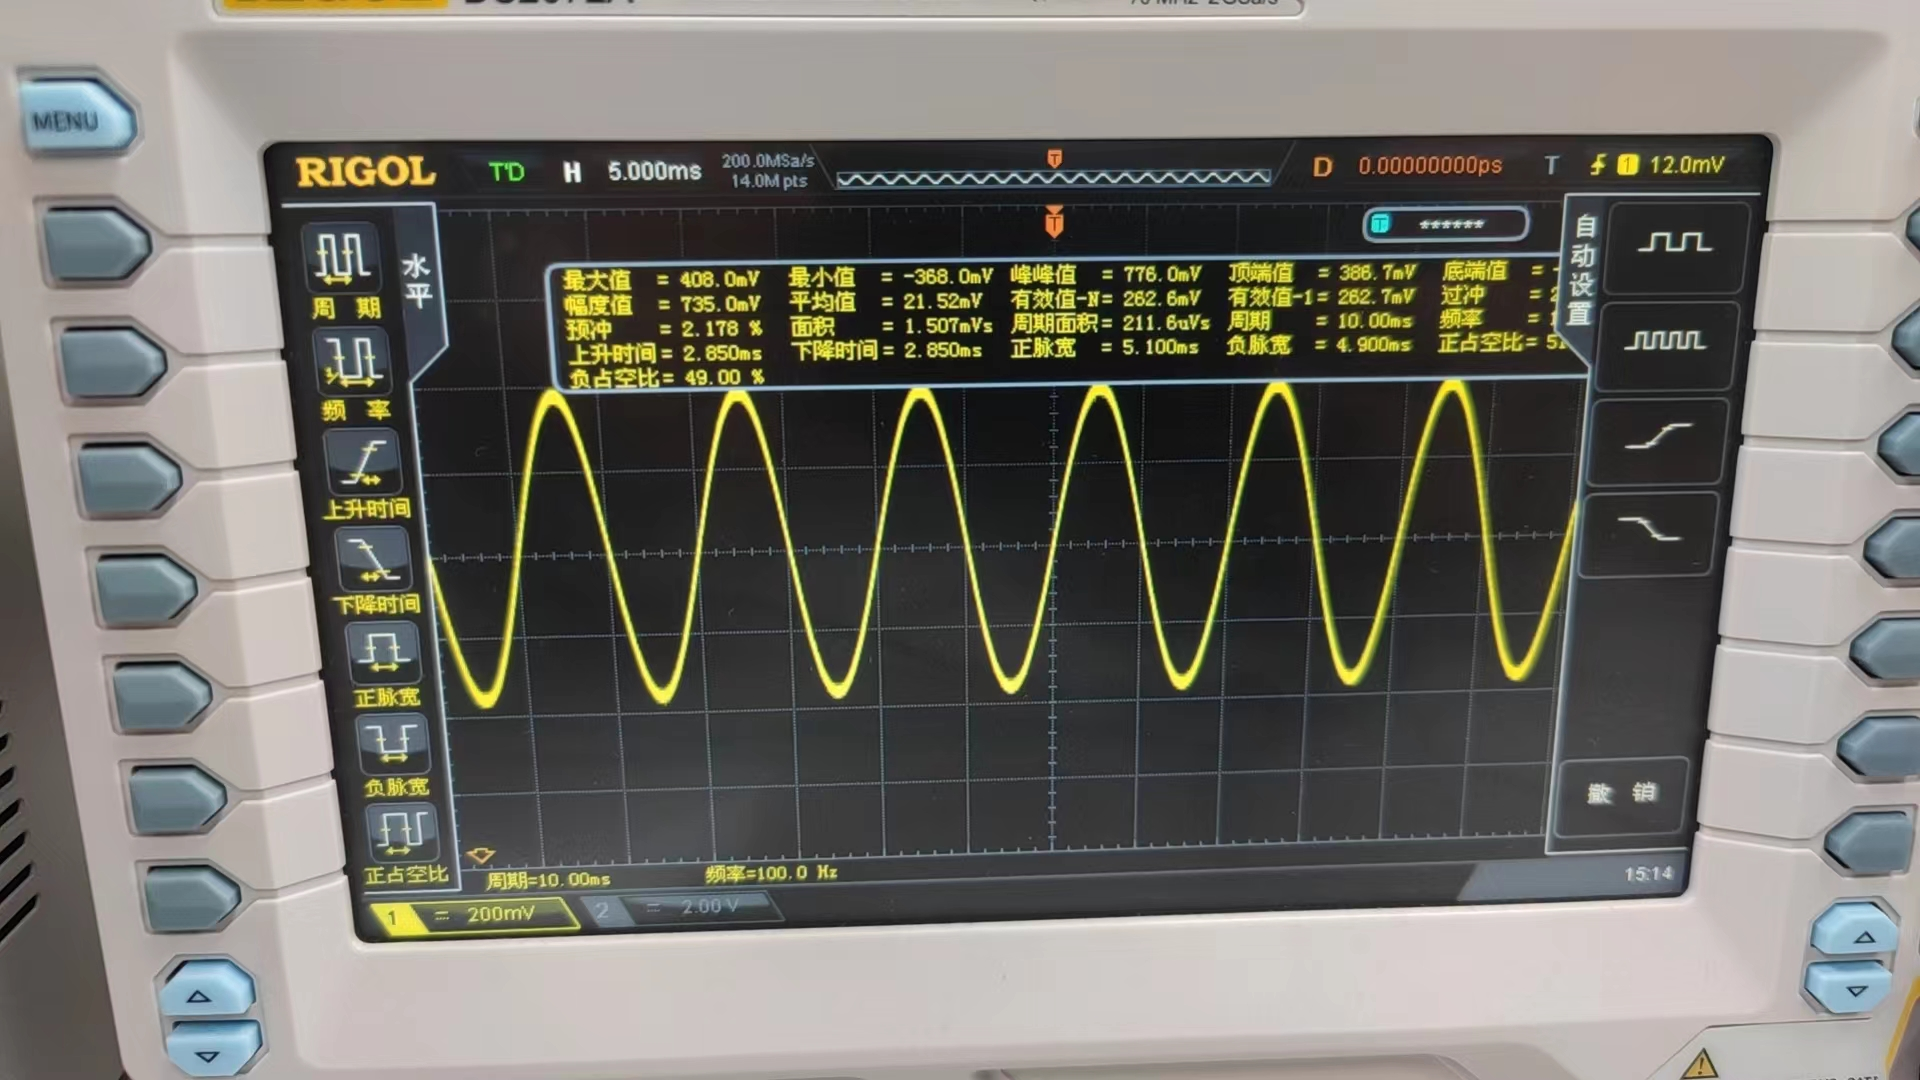
\includegraphics[width=0.9\linewidth]{低通滤波100Hz}%%%%%%%%%note3
			\caption{低通滤波100Hz}
			\label{低通滤波100Hz}
		\end{minipage}%
		\begin{minipage}[t]{0.49\linewidth}%%%%%%%%%note2
			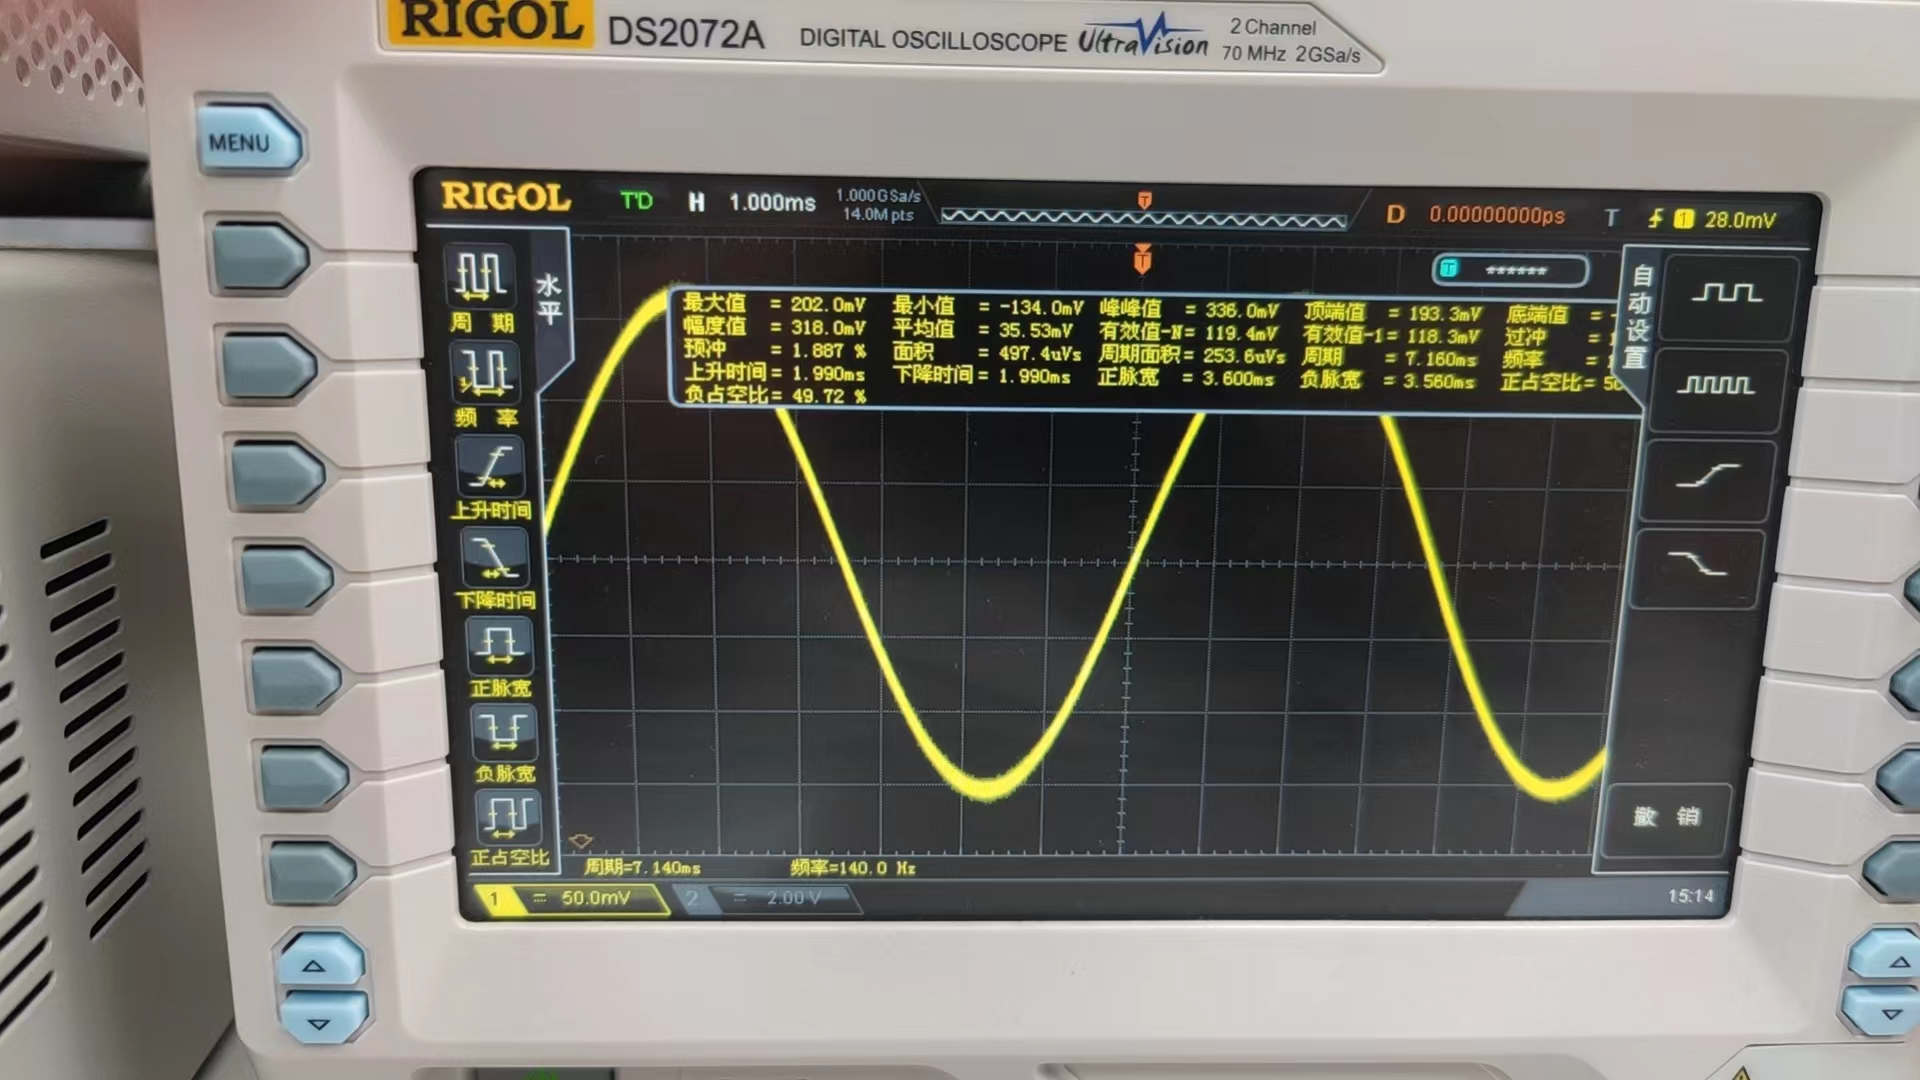
\includegraphics[width=0.9\linewidth]{低通滤波140Hz}%%%%%%%%%note3
			\caption{低通滤波140Hz}
			\label{低通滤波140Hz}
		\end{minipage}%
	\end{figure}

	\begin{table}[htbp]
		\centering
		\begin{tabular}{ c|c|c|c|c|c|c|c p{1.5cm}|}
			\hline
			频率(Hz) & 20 & 40 & 60 & 80 & 100 & 120 & 140 \\
			\hline
			峰峰值(V)  & 1.380 & 1.328 & 1.248 & 1.040 & 0.776 & 0.528 & 0.336 \\
			\hline
		\end{tabular}
		\caption{低通滤波20Hz到140Hz测量结果}\label{低通滤波20Hz到140Hz测量结果}
	\end{table}

	我们将表中的测试结果绘制成曲线图,能够更好地看出低通滤波的效果,曲线图如图\ref{低通滤波}所示。从曲线图中,我们可以看出该低通滤波器是可以正常工作、达到低通滤波的效果,并且当其峰峰值下降至-3dB时,频率为84Hz左右,所以该低通滤波器的效果还是不错的,带外的抑制效果也能达到要求。
	
	\begin{figure}[h]
		\centering%使该部分内容居中
		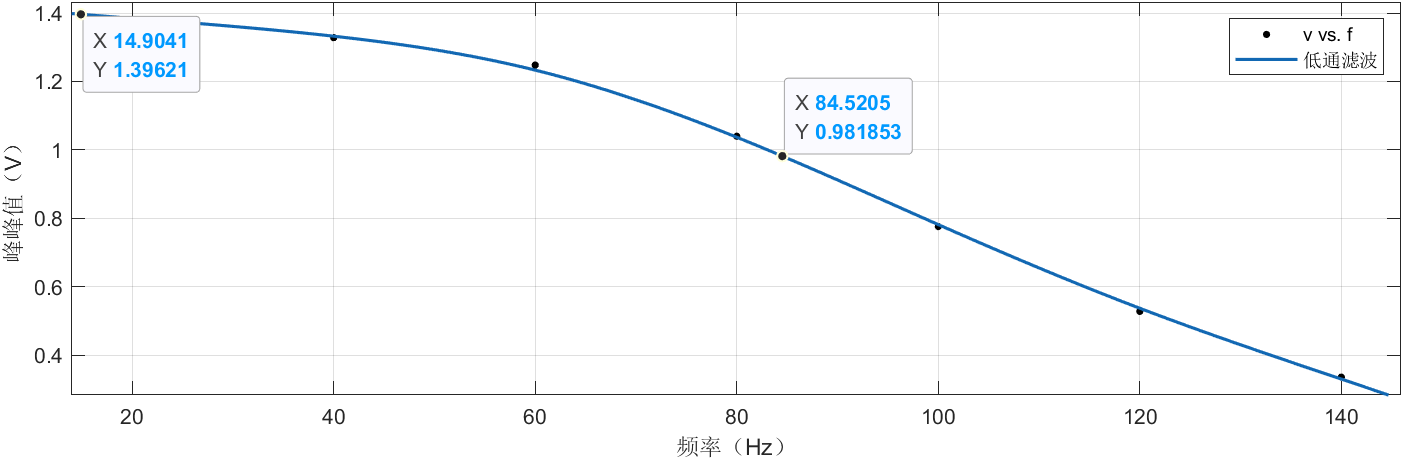
\includegraphics[width=6in]{低通滤波}
		\caption{低通滤波}%命名并编号
		\label{低通滤波}%设置标签
	\end{figure}

	
	\subsubsection{高通滤波部分}

	\begin{figure}[H]
		\centering
		\begin{minipage}[t]{0.4\linewidth}%%%%%%%%%note2
			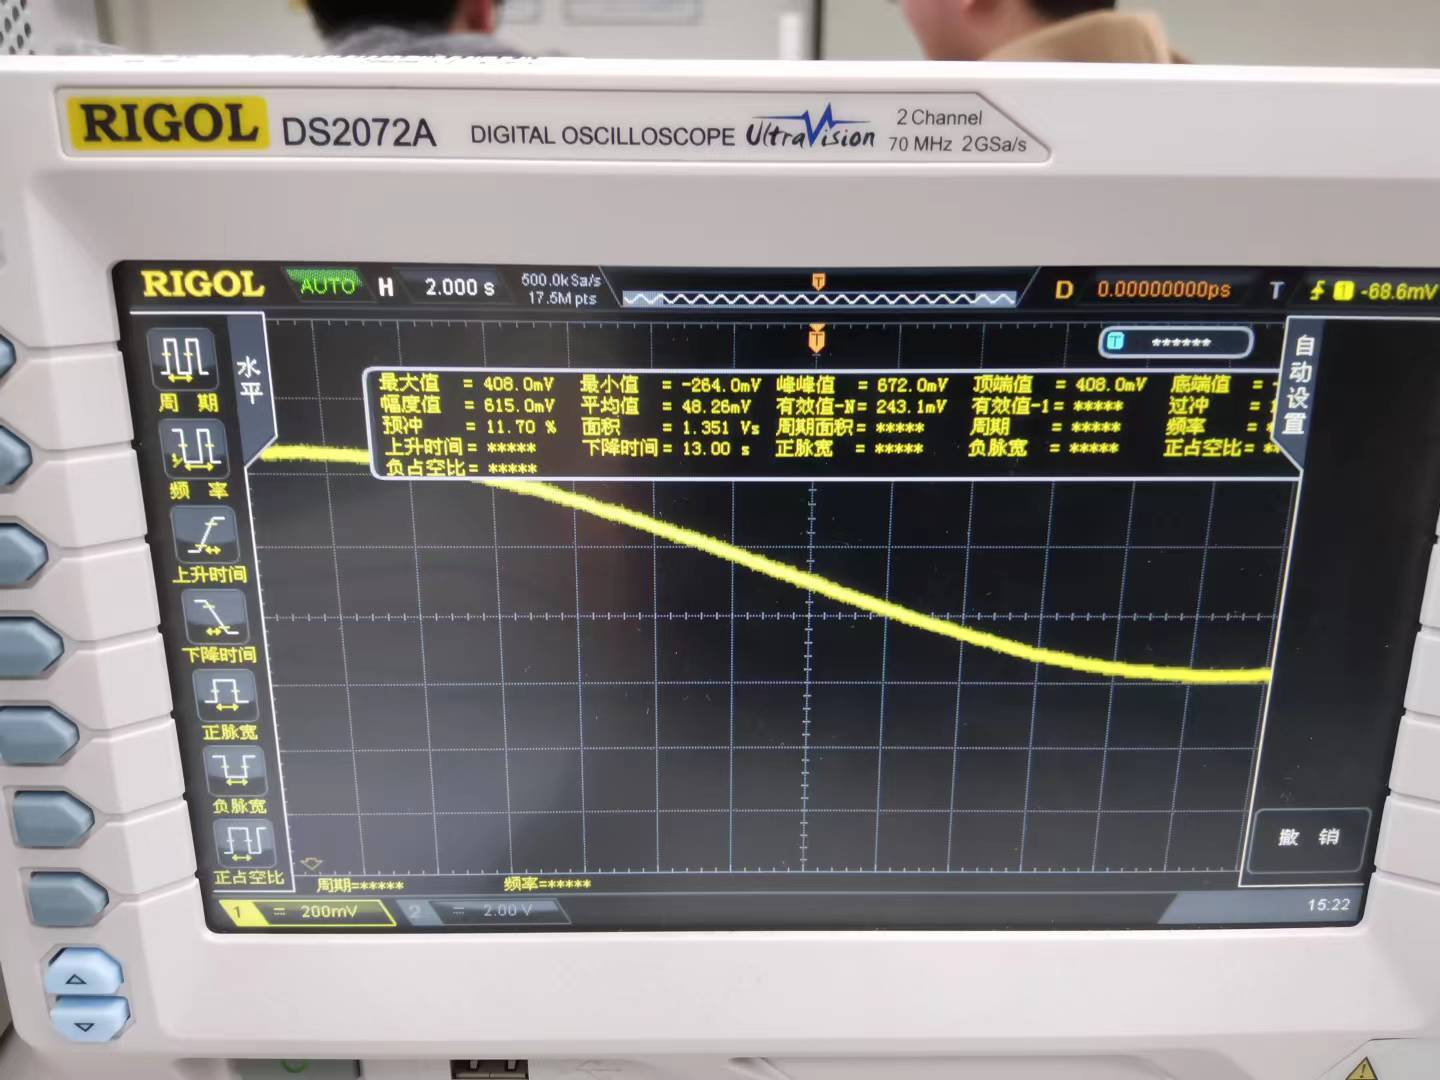
\includegraphics[width=0.9\linewidth]{高通滤波20mHz}%%%%%%%%%note3
			\caption{高通滤波20mHz}
			\label{高通滤波20mHz}
		\end{minipage}%
		\begin{minipage}[t]{0.4\linewidth}
			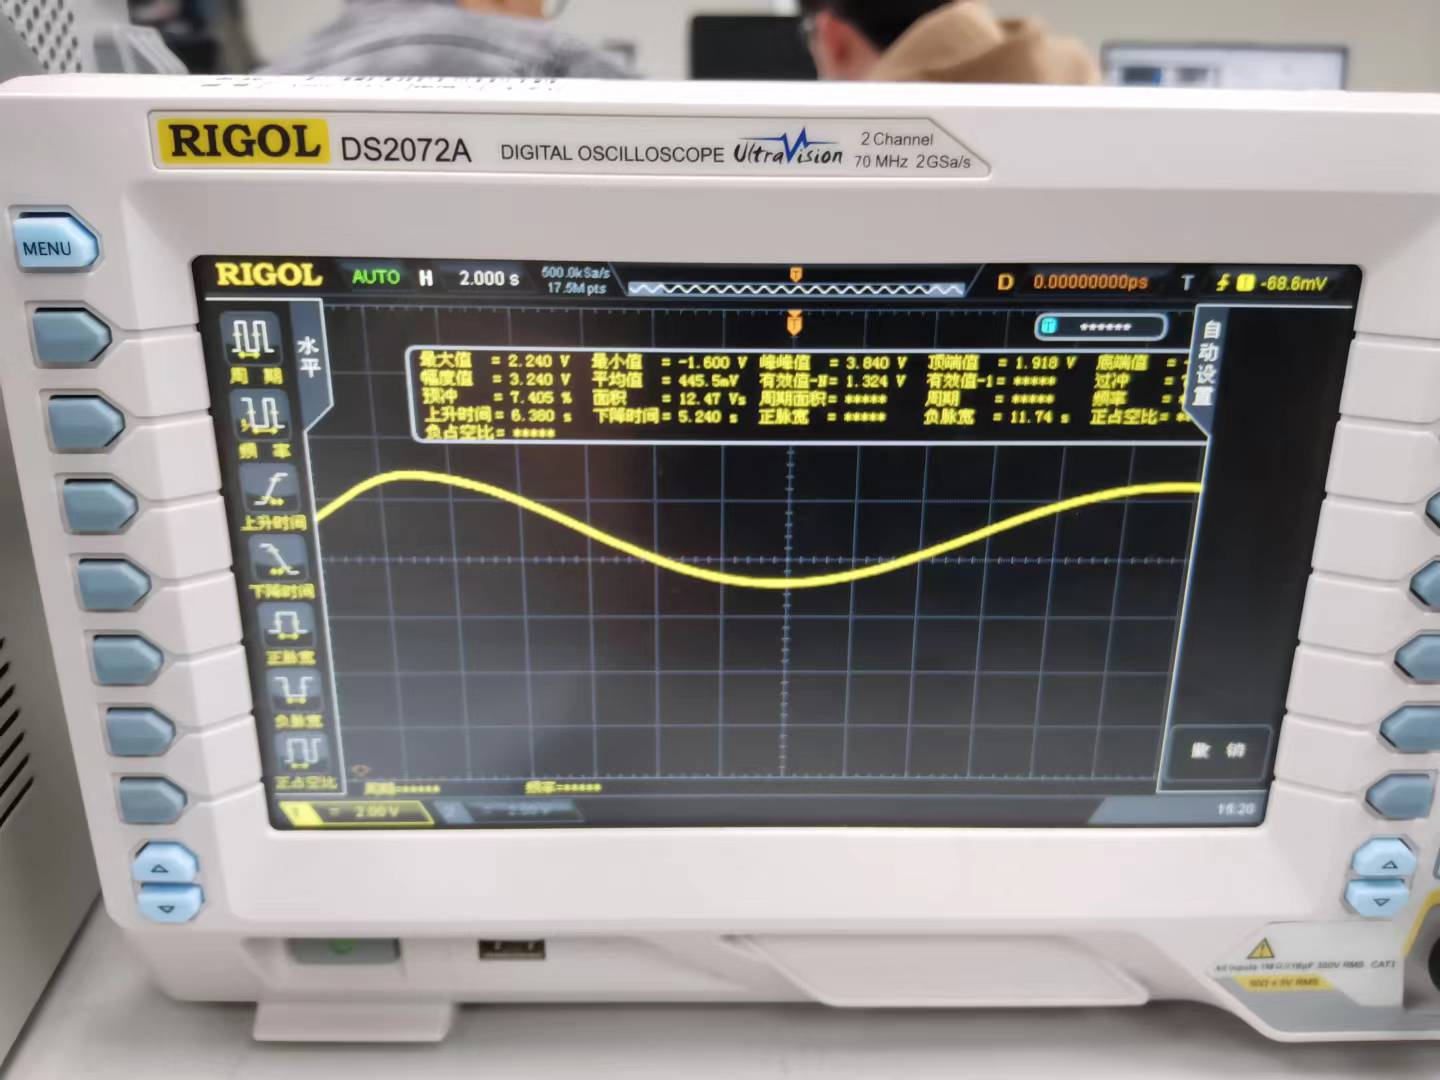
\includegraphics[width=0.9\linewidth]{高通滤波40mHz}
			\caption{高通滤波40mHz}
			\label{高通滤波40mHz}
		\end{minipage}
		
		\begin{minipage}[t]{0.4\linewidth}%%%%%%%%%note2
			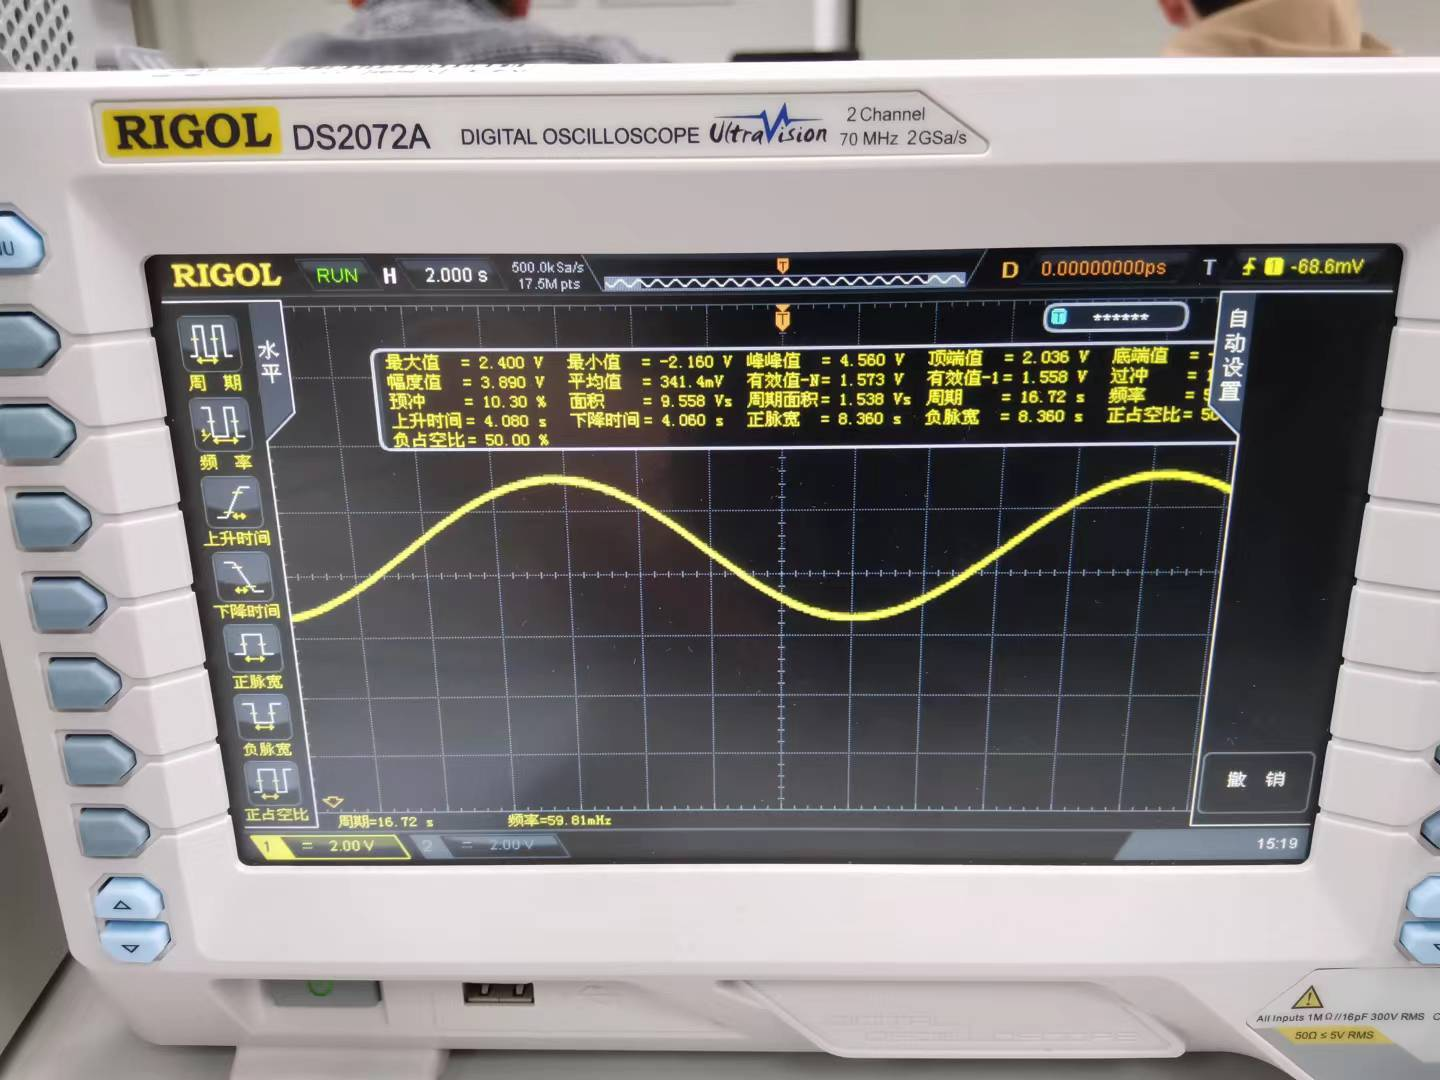
\includegraphics[width=0.9\linewidth]{高通滤波60mHz}%%%%%%%%%note3
			\caption{高通滤波60mHz}
			\label{高通滤波60mHz}
		\end{minipage}%
		\begin{minipage}[t]{0.4\linewidth}%%%%%%%%%note2
			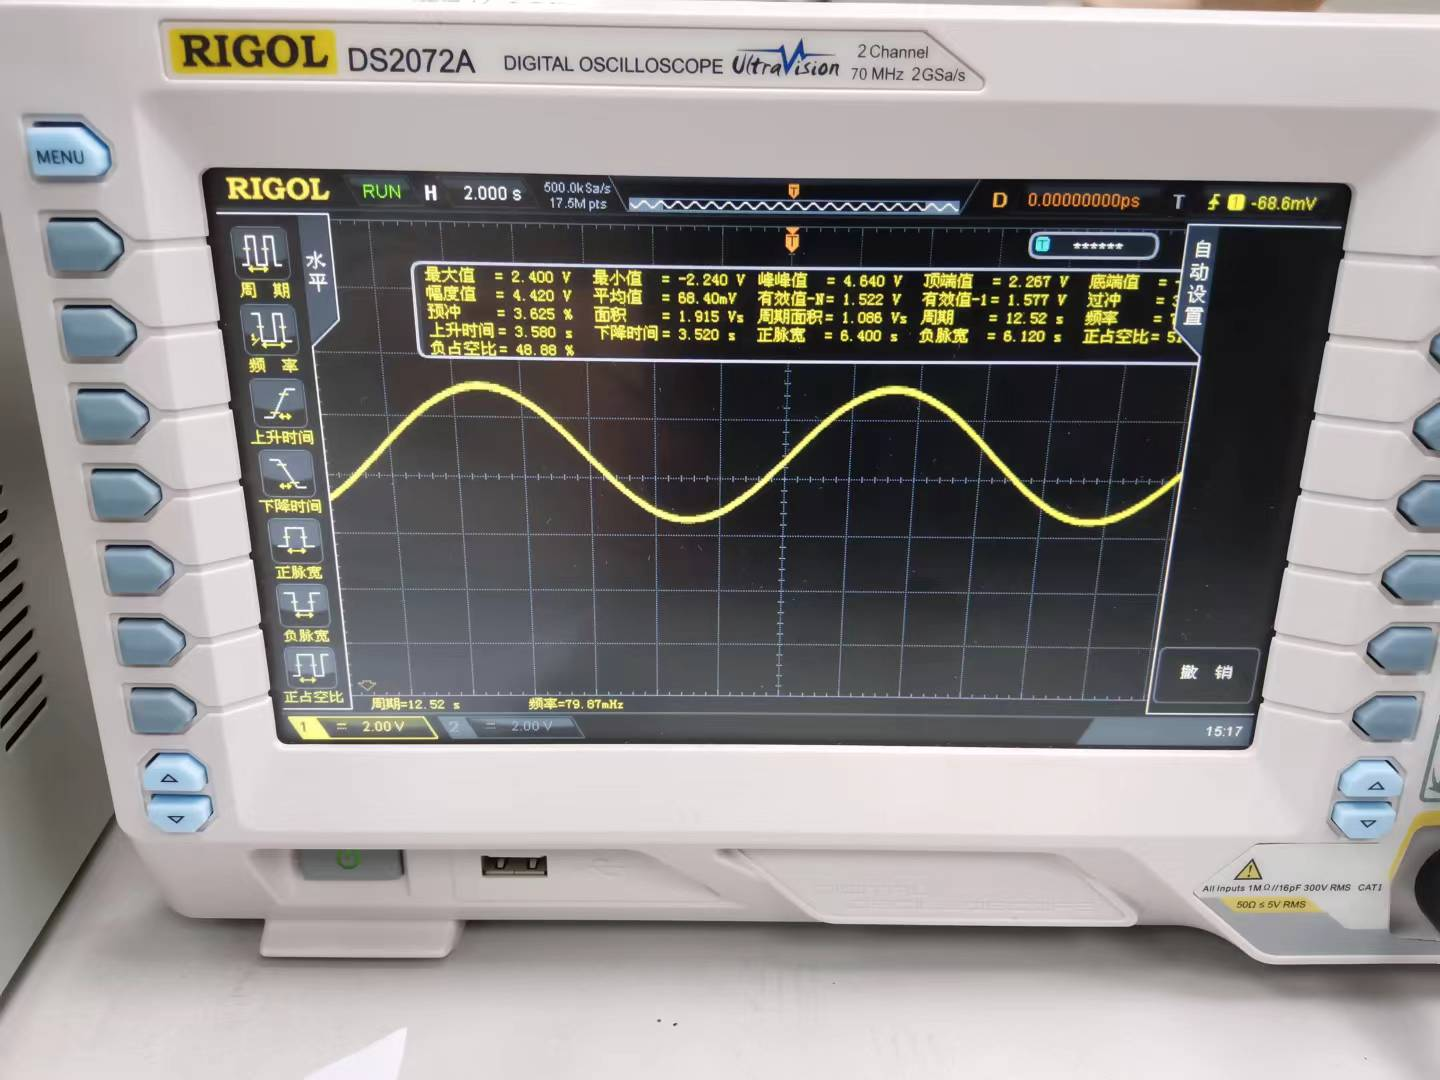
\includegraphics[width=0.9\linewidth]{高通滤波80mHz}%%%%%%%%%note3
			\caption{高通滤波80mHz}
			\label{高通滤波80mHz}
		\end{minipage}%
	\end{figure}

	在测试高通滤波部分时,主要针对20mHz到80mHz部分,测试图如图\ref{高通滤波20mHz}、\ref{高通滤波40mHz}、\ref{高通滤波60mHz}、\ref{高通滤波80mHz}所示,测试的数据如表\ref{高通滤波20mHz到100mHz测量结果}所示。将测试数据绘制成图像,能得到如图\ref{高通滤波}所示的曲线图。
	
	\begin{table}[htbp]
		\centering
		\begin{tabular}{ c|c|c|c|c p{1.5cm}}
			\hline
			频率(mHz) & 20 & 40 & 60 & 80  \\
			\hline
			峰峰值(V)  & 0.672 & 3.840 & 4.560 & 4.640 \\
			\hline
		\end{tabular}
		\caption{高通滤波20mHz到100mHz测量结果}\label{高通滤波20mHz到100mHz测量结果}
	\end{table}
	
	\begin{figure}[h]
		\centering%使该部分内容居中
		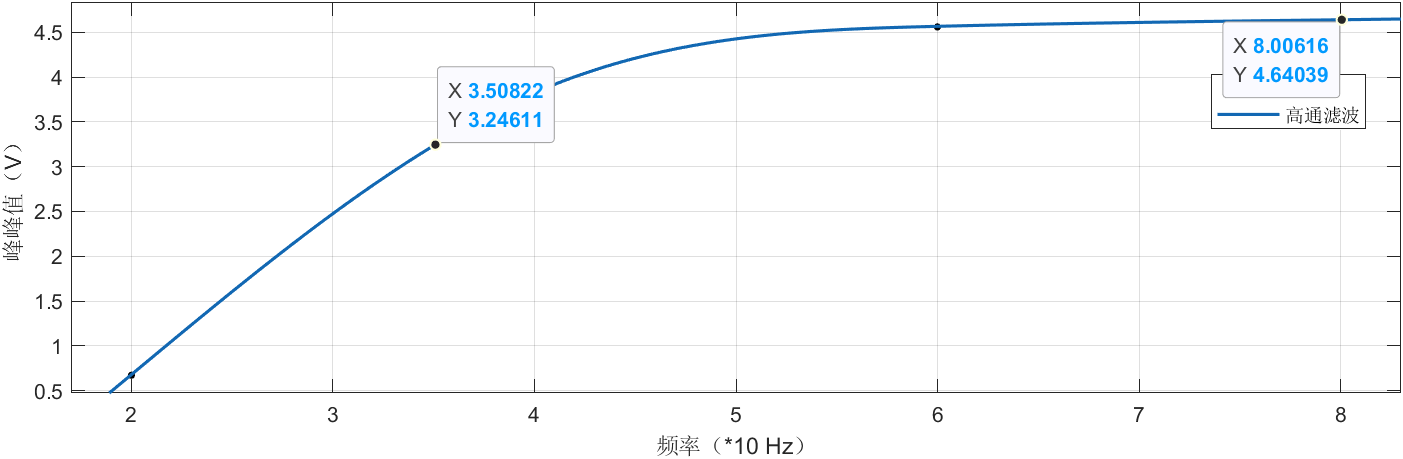
\includegraphics[width=6in]{高通滤波}
		\caption{高通滤波}%命名并编号
		\label{高通滤波}%设置标签
	\end{figure}

	从图中,我们能看出,高通滤波器能够正常工作并起到滤波的效果,当其峰峰值下降为-3dB时,频率约为35mHz,基本满足需求,同时带外抑制的效果也比较好。
	
	\subsubsection{陷波部分}
	
	在陷波部分,我们为得到陷波的频率,设置了从50Hz到35Hz的测试范围,如图\ref{陷波最低点}所示是测试时峰峰值最低点的图像。最终得到的测试数据如表\ref{陷波测试结果}所示。根据表中测试数据,我们绘制出陷波曲线,如图所示,能够更好地看出陷波地效果。
	
	\begin{figure}[H]
		\centering%使该部分内容居中
		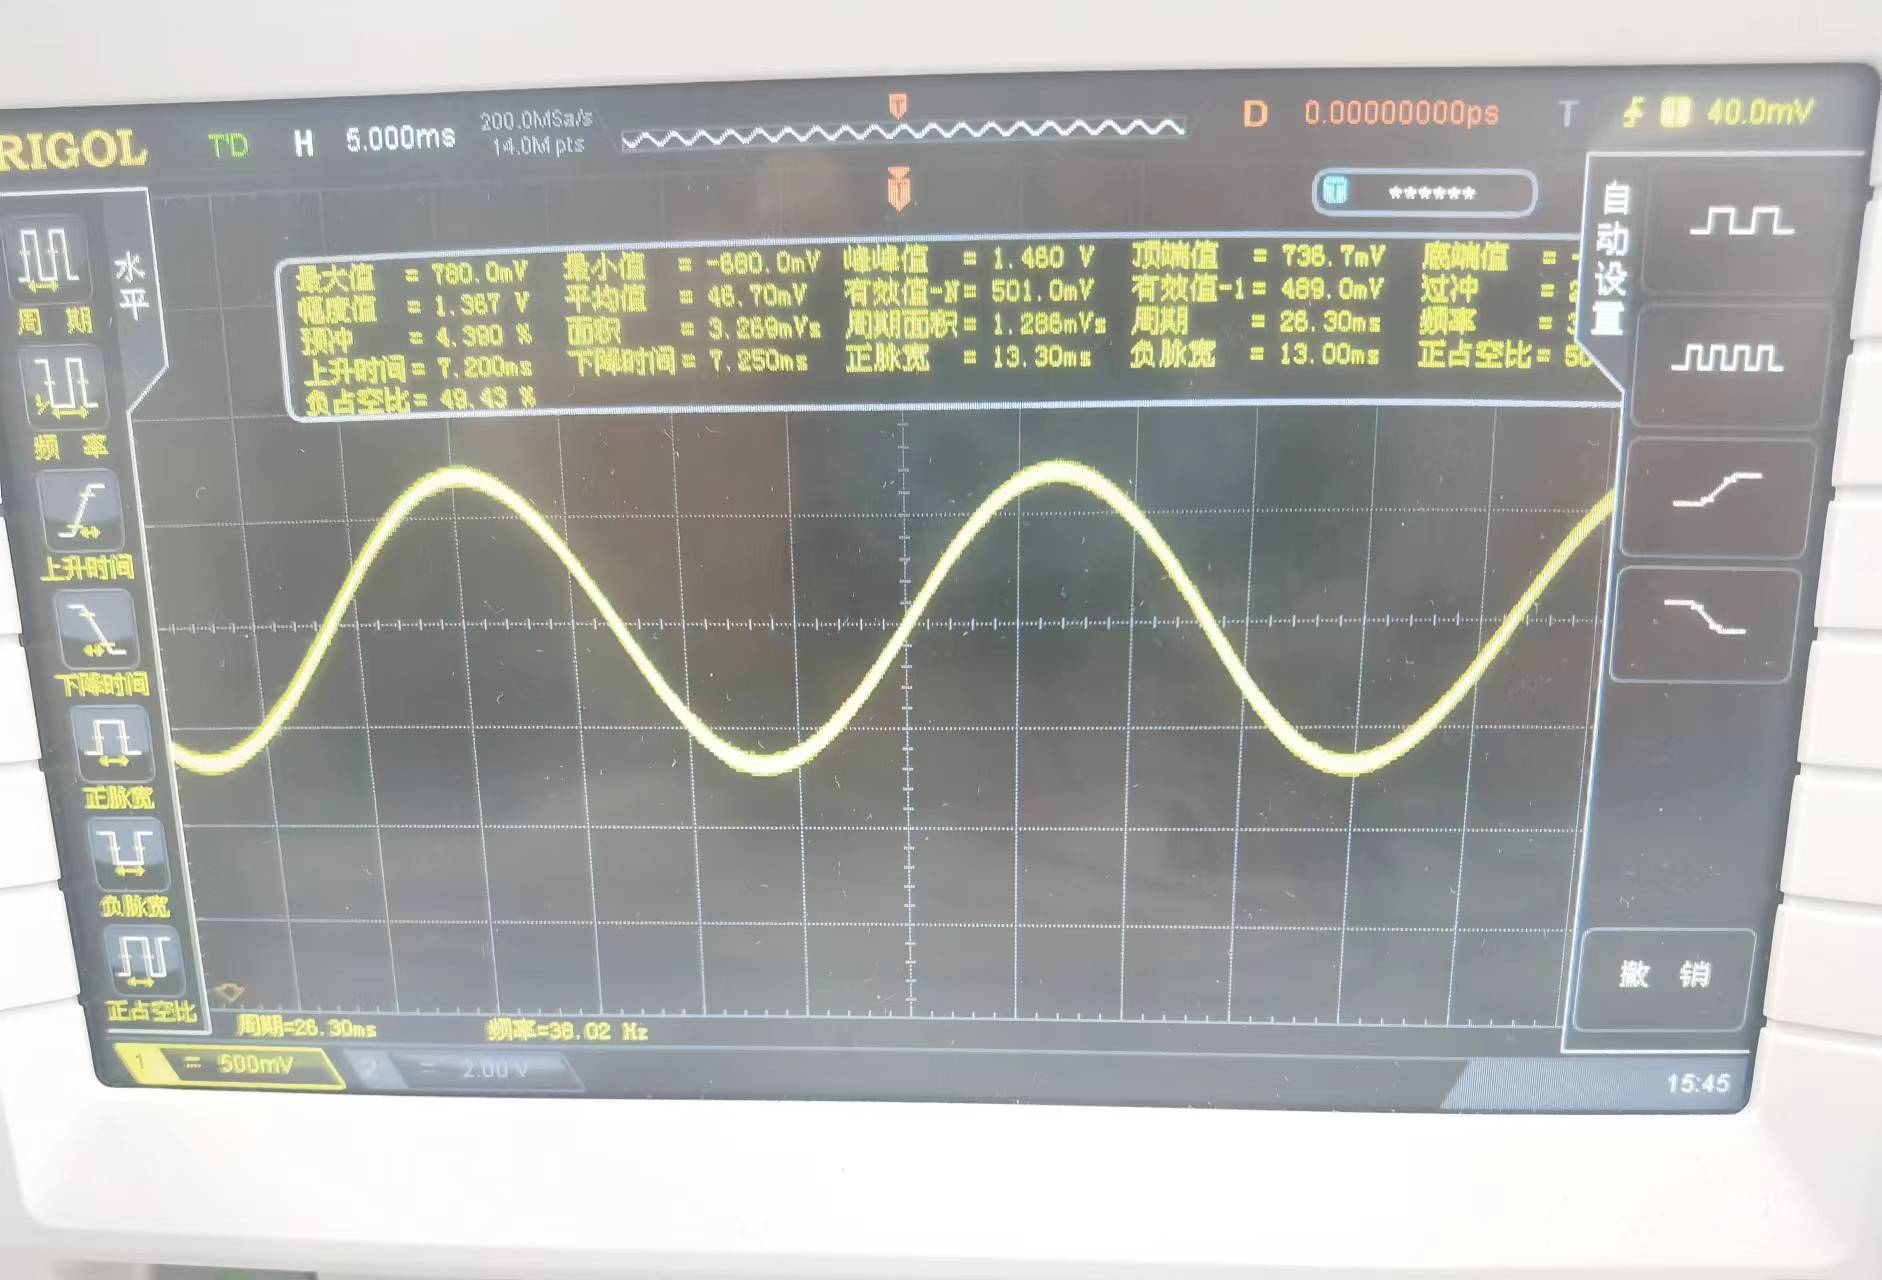
\includegraphics[width=3in]{陷波最低点}
		\caption{陷波最低点}%命名并编号
		\label{陷波最低点}%设置标签
	\end{figure}
	
	\begin{table}[htbp]
		\centering
		\begin{tabular}{ c|c|c|c|c|c|c|c|c p{1.5cm}}
			\hline
			频率(Hz) & 50 & 49 & 48 & 47 & 46 & 45 & 44 & 43  \\
			\hline
			峰峰值(V)  & 3.040 & 2.960 & 2.840 & 2.720 & 2.600 & 2.480 & 2.300 & 2.140 \\
			\hline
		\end{tabular}
	\end{table}

	\begin{table}[H]
		\centering
		\begin{tabular}{ c|c|c|c|c|c|c|c p{1.5cm}}
			\hline
			 42 & 41 & 40 & 39 & 38 & 37 & 36 & 35  \\
			\hline
			 1.980 & 1.800 & 1.640 & 1.560 & 1.460 & 1.520 & 1.640 & 1.880 \\
			\hline
		\end{tabular}
		\caption{陷波测试结果}\label{陷波测试结果}
	\end{table}

	\begin{figure}[H]
		\centering%使该部分内容居中
		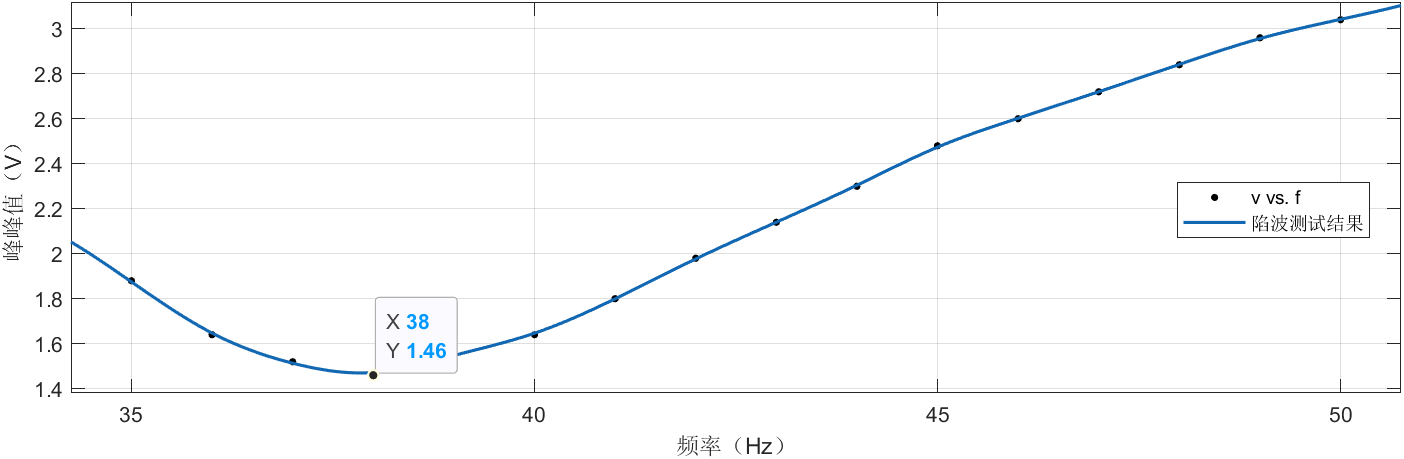
\includegraphics[width=6.5in]{陷波测试结果}
		\caption{陷波测试结果}%命名并编号
		\label{陷波测试结果图}%设置标签
	\end{figure}

	从图中,我们可以看出,陷波的中心位置为38Hz,更细致应该是在37到38Hz之间,而我们希望的陷波位置应该为40到50Hz之间,且该滤波测试结果中,陷波地带宽比较大,合格的陷波器的陷波位置应该是比较窄的,因此,陷波部分地效果并不理想。效果不理想的原因,最主要的应该是焊接使用的电容的电容值偏离指定值,导致陷波位置发生了偏移。
	
	\subsubsection{总体放大性能}
	
	在心电信号处理电路各个单独部分测试完成后,我们进行电路总体放大性能的测试,设置了20Hz到140Hz的测试范围,其测试结果如表\ref{总体性能测试结果}所示。根据表中数据,绘制得到如图\ref{总体放大性能}所示的曲线。
	
	\begin{table}[htbp]
		\centering
		\begin{tabular}{ c|c|c|c|c|c|c|c|c|c|c|c|c|c p{1.5cm}}
			\hline
			频率(Hz) & 20 & 30 & 40 &50 & 60 &70 & 80 &90 & 100 & 110 & 120 &130 & 140 \\
			\hline
			峰峰值(V)  & 2.580 & 2.120 & 0.900 & 1.780 & 2.160 & 2.200 & 2.060 & 1.840 & 1.580 & 1.380 & 1.140 & 0.960 & 0.752 \\
			\hline
		\end{tabular}
		\caption{总体性能测试结果}\label{总体性能测试结果}
	\end{table}

	\begin{figure}[H]
		\centering%使该部分内容居中
		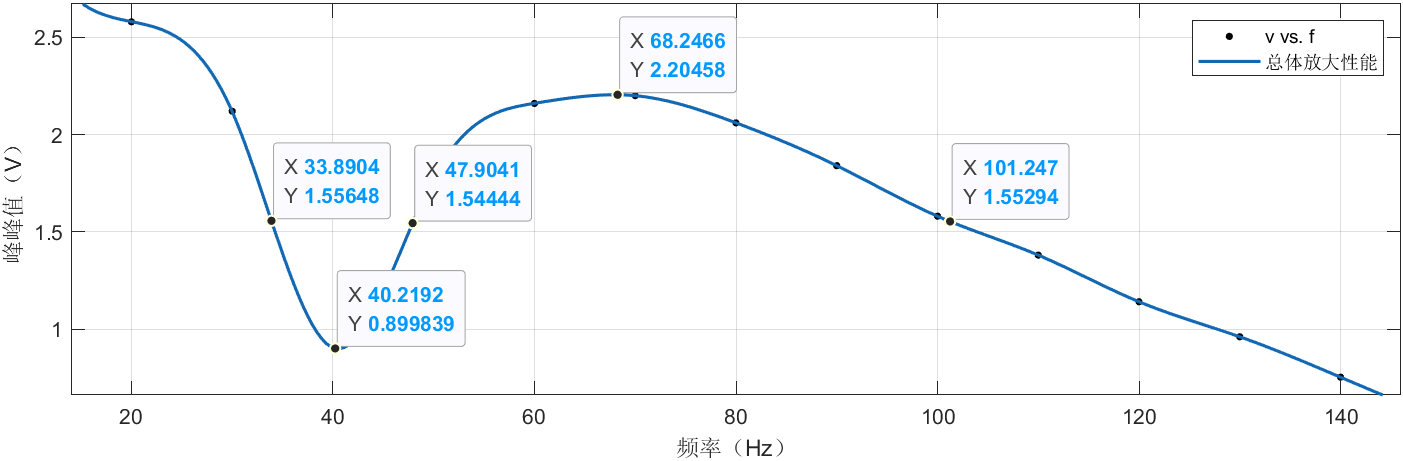
\includegraphics[width=6.5in]{总体放大性能}
		\caption{总体放大性能}%命名并编号
		\label{总体放大性能}%设置标签
	\end{figure}

	从图中可以看出,在40Hz左右发生陷波,在30Hz之前和45到101Hz之间增益较高,其余位置的抑制都较为明显,基本符合我们设计的初衷,能够起到总体处理和放大心电信号的作用。
	
	\subsubsection{人体测试}
	
	在测试完ECG信号检测调理电路的各类参数性能之后,我们进行人体测试,观察该电路实际能否起到处理心电信号,最终输出合格波形的作用。测试结果如图所示。
	
	\begin{figure}[H]
		\centering%使该部分内容居中
		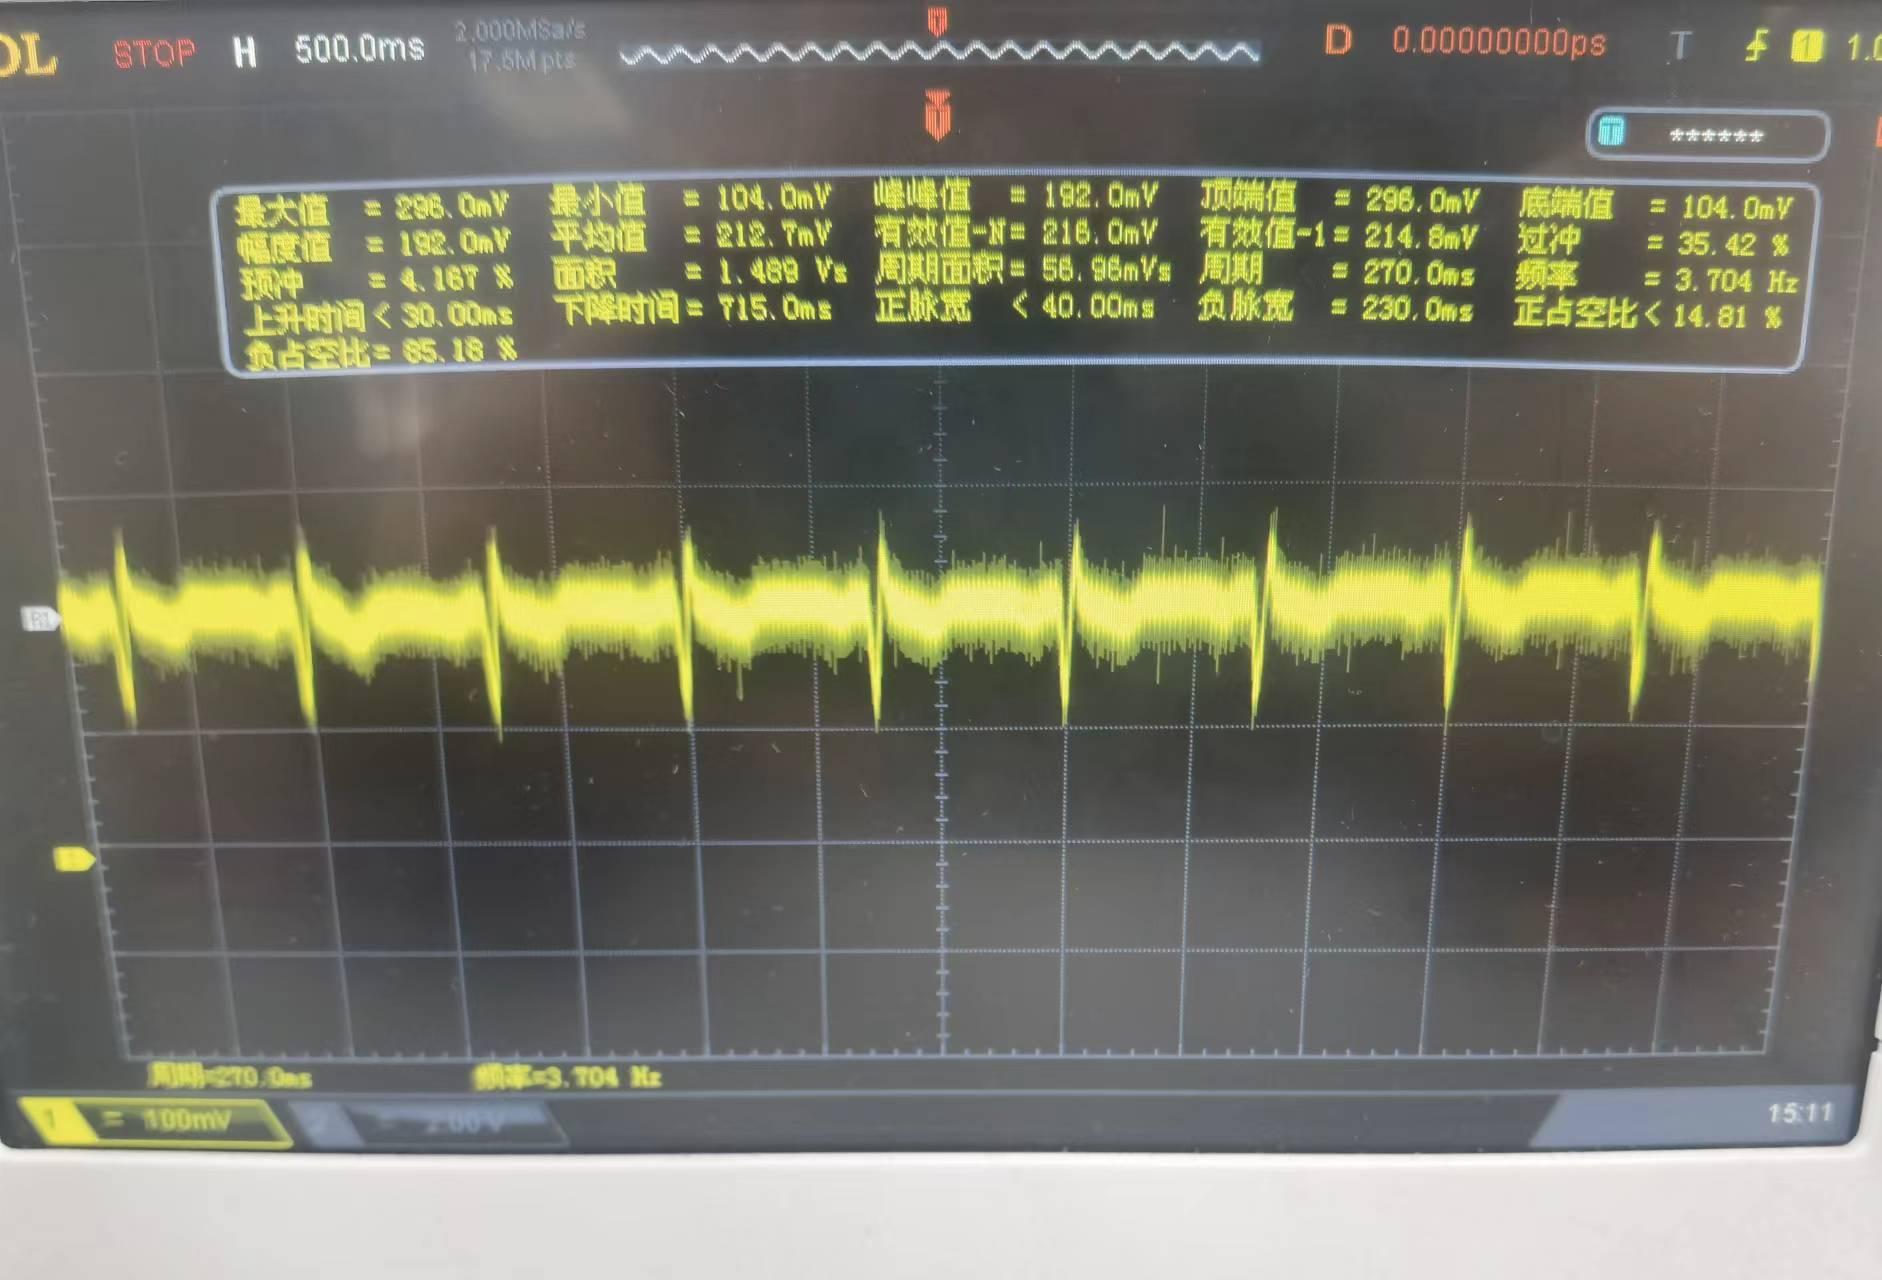
\includegraphics[width=4in]{ECG信号检测调理电路_人体测试}
		\caption{ECG信号检测调理电路-人体测试}%命名并编号
		\label{ECG信号检测调理电路_人体测试}%设置标签
	\end{figure}

	在示波器上,我们已经可以看出心电信号的波形,但同时,也发现其中混叠的杂波较多,心跳与心跳之间干扰明显,心电信号的增益还不够大,容易和杂波混在一起。
	
	\section{ECG心电监测系统}
	
	\subsection{总体目标}
	
	
	
	\subsubsection{系统框图及功能说明}
	
	\subsection{硬件设计与调试}
	
	\subsubsection{原理图设计}
	
	\subsubsection{PCB设计}
	
	\subsubsection{硬件调试}
	
	\subsubsection{硬件电路整体性能分析}
	
	\subsection{软件设计与调试}
	
	\subsubsection{软件工作流程框图}
	
	\subsubsection{软件功能设计}
	
	\subsubsection{软件调试}
	
	\section{总结}
	
	\subsection{韩寒:}
	
	\subsection{谌梓轩:}
	
	
\end{document}